
%(BEGIN_QUESTION)
% Copyright 2010, Tony R. Kuphaldt, released under the Creative Commons Attribution License (v 1.0)
% This means you may do almost anything with this work of mine, so long as you give me proper credit

A guided-wave radar transmitter is installed in this process vessel through a nozzle welded to the vessel at a 35$^{o}$ angle from horizontal:

$$\includegraphics[width=15.5cm]{i03744x01.eps}$$

This transmitter's rigid probe happens to be precisely 8 feet 0 inches long, and has transition zones 20 inches in length (each).  Calculate the {\it vertical} level-measurement span this transmitter will provide as installed.

\underbar{file i03744}
%(END_QUESTION)





%(BEGIN_ANSWER)

Vertical measurement span = 2 feet 8 inches

%(END_ANSWER)





%(BEGIN_NOTES)


%INDEX% Measurement, level: radar

%(END_NOTES)

